\begin{figure}[h!]
	\centering
	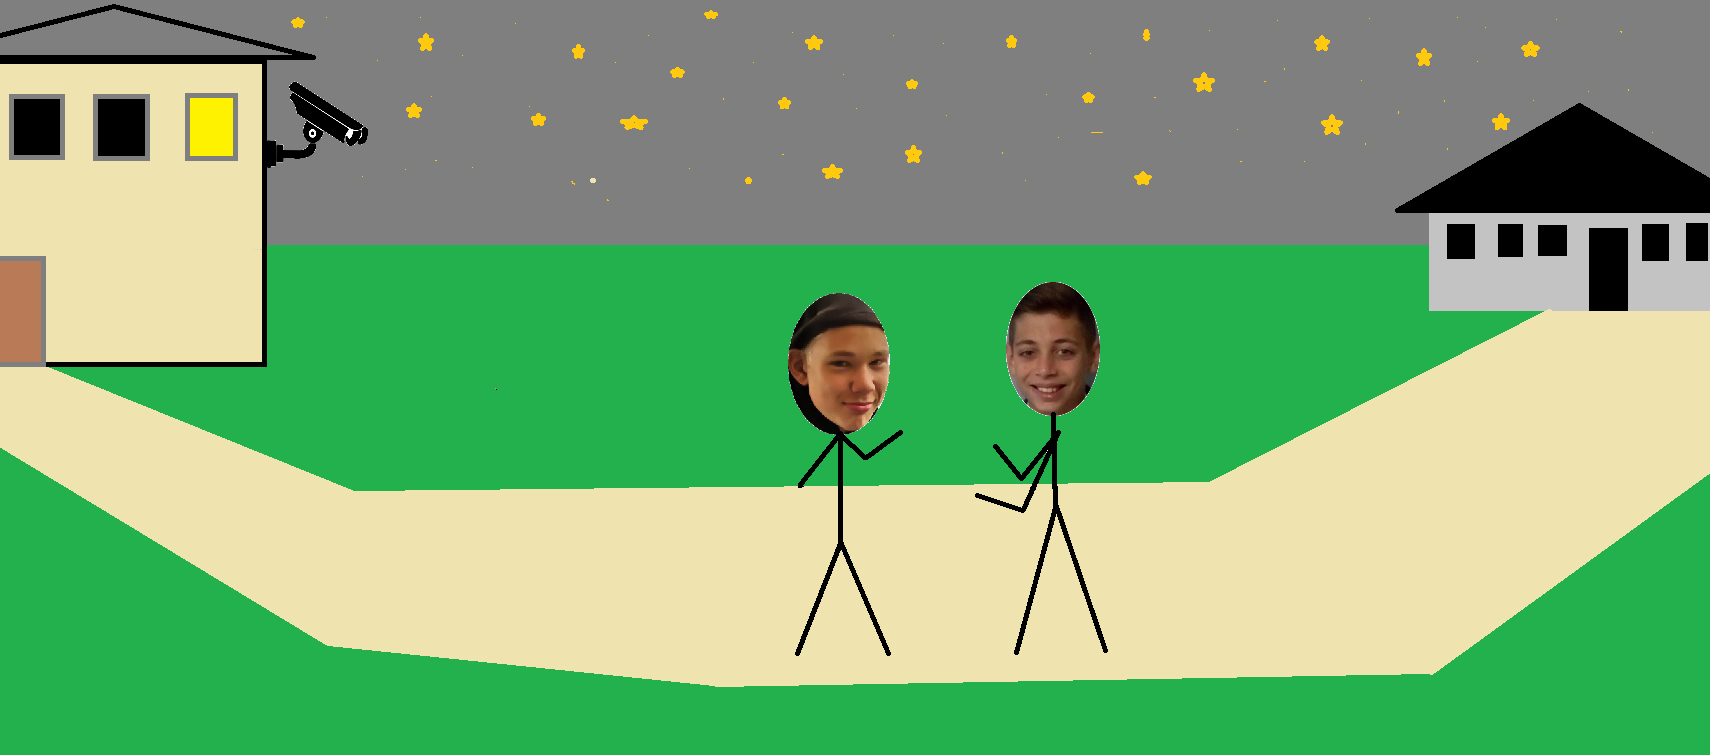
\includegraphics[width=0.8\linewidth, keepaspectratio]{boys.png}
\end{figure}

В том же самом далеком лагере, но уже не в той же самой далекой усадьбе, 
а в небольшом домике у реки собрались как-то ночью два закадычных друга~---~Рамаз и мальчик, не имеющий имени, известный под прозвищем Кругляк. 
Болтали они, болтали, но поняли, что сна нет ни в одном глазу, а темы для разговора заканчиваются~---~и девчонок, что мирно спали в соседней комнате обсудили, 
и вредных вожатых, и нерешаемые задачи на занятиях. И решили они выйти воздухом свежим подышать, да погулять под звездами. 
Но так как лагерь был со строгими правилами, за детьми круглосуточно следили множество видеокамер, которые отслеживали каждый шаг детишек. 
Мальчик без имени знал от своих соотрядцев, что жили в той самой усадьбе, что видеокамеры не могли каждую секунду следить за всей территорией. 
Те ребята, кто был сослан в лагерь не в первый раз, уже смогли на собственном опыте выявить закономерность~---~для этого они разделили 
всю территорию между футбольным полем и усадьбой на последовательные прямоугольники и каждому присвоили значение видимости 
(чем больше значение, тем реже камеры  следят за данным участком, чем меньше число~---~тем больше шанс попасться). 
Прямоугольники имели ширину в полшага. За раз ребята могли сдвинуться либо на полшага, либо сделать целый шаг. 
После появления в новом прямоугольнике, ребята записывали сумму значений видимости предыдущих посещенных прямоугольников.
Необходимо помочь ребятам не засветится на камерах~---~для этого необходимо определить самый безопасный способ прохода до усадьбы 

\InputFile
\noindent

На первой строке задается количество прямоугольников $K (1 \leq K \leq 100)$.
На второй строке - степень видимости в прямоугольнике $P_i (-20 \leq P_i \leq 20)$.

\OutputFile
\noindent

Вывести результат~---~максимальная возможная сумма значений видимости в прямоугольнике $P_K$ (т.е нужно пройти такой путь, чтобы в последнем прямоугольнике была максимальная сумма по всему пройденному пути). 

\SAMPLES